
\documentclass[conference]{IEEEtran}
\usepackage{amsmath}
\usepackage{amssymb}
\usepackage{graphicx}
\usepackage{cite}
\usepackage{color}
\usepackage{url}
\usepackage{algorithm}
\usepackage{algorithmic}
\usepackage{booktabs}
\usepackage{multirow}
\usepackage{hyperref}
\graphicspath{{figures/}}

\begin{document}

\title{Persistent Note-Based Memory for LLM Agents: A Pilot Study of Cost, Retention, and Scaling Limits}

\author{\IEEEauthorblockN{Ishan Gautam}
\IEEEauthorblockA{
\textit{Pulchowk Campus} \\
\textit{Institute of Engineering, Tribhuvan University} \\
Lalitpur, Nepal \\
080bct034.ishan@pcampus.edu.np
}
\and
\IEEEauthorblockN{Kushal K.C.}
\IEEEauthorblockA{
\textit{Pulchowk Campus} \\
\textit{Institute of Engineering, Tribhuvan University} \\
Lalitpur, Nepal \\
080bct041.kushal@pcampus.edu.np
}
}

\maketitle

\begin{abstract}
Large language model (LLM) agents incur token costs that grow super-linearly with conversation length because each step may re-send an expanding history. Persistent external memory is often proposed as a remedy, but its retention/cost trade-off is easy to overstate. This paper studies \emph{persistent note-based memory}, a hierarchical architecture in which a small model extracts structured memory from conversation segments and a larger model answers from that memory plus a recent-message window. We formalize the cost model, specify two concrete memory representations, release a reproducible evaluation harness, and report pilot live evaluations against full-context, truncation, and running-summary baselines. The initial append-only notes result is mixed rather than validating: across two Groq reruns on synthetic fact-tracking conversations (16 total cases, up to 56 messages), hierarchical notes cost 102.7\% of full context while retaining 69.4\% of planted facts. We then evaluate a latest-value fact-slot variant that overwrites subject--predicate facts instead of appending all extracted notes. In a second two-seed live pilot (16 cases), fact-slot memory reduces real input tokens by 40.9\%, retains 85.2\% of planted facts, and costs 89.1\% of full context; however, full context still retains more facts (95.6\%) and update retention remains weaker for slots (71.9\%). A cheap-vs-expensive extractor ablation for append-only notes is inconclusive (69.4\% vs. 68.2\% retention with overlapping intervals). Separately, a deterministic token-accounting simulation suggests that bounded notes could reduce cost to 13.0\% of full-context cost at 480 messages, but that simulation does not measure live retention under compaction. We therefore present the system as a transparent pilot: structured persistent memory can improve the cost/retention frontier over append-only notes, but the evidence remains small-scale and motivates larger paired long-horizon experiments.
\end{abstract}

\begin{IEEEkeywords}
large language model agents, LLM cost optimization, conversation summarization, persistent memory, model cascading, token-efficient prompting, hierarchical memory, long-context management, prompt compression, retrieval-augmented memory, agentic systems
\end{IEEEkeywords}

\section{Introduction}

Autonomous AI agents have revolutionized tasks ranging from market intelligence to sales outreach, yet their economic viability remains challenged by escalating token costs. Unlike traditional chat applications where a single query consumes approximately 1,000 tokens, autonomous agents perform multi-step reasoning, tool calls, and context re-stacking, consuming 20,000 to 100,000 tokens minimum per task \cite{zhou2024agents, park2023generative}.

The problem intensifies as conversations lengthen. As agents carry more history behind each step, the cumulative token cost over a multi-turn task grows quadratically rather than linearly. Poorly architected agents can consume resources at unsustainable rates once realistic retry rates, parallel instances, and tool overhead are accounted for \cite{shinn2023reflexion}. Worse, simply enlarging the context window is not a free remedy: long-context models exhibit a ``lost in the middle'' effect, where information placed away from the beginning or end of a long prompt is poorly utilized \cite{nfliu2023lost}, and the self-attention mechanism makes each additional token quadratically expensive in compute \cite{packer2023memgpt}.

Current mitigation strategies include:
\begin{enumerate}
    \item \textbf{Semantic Caching}: Reuse outputs for semantically similar inputs \cite{bang2023gptcache}.
    \item \textbf{History Summarization}: Compress past conversations into running summaries to bound context length \cite{acl2024}.
    \item \textbf{Model Cascading}: Use small models for easy sub-tasks and escalate to expensive models only when required \cite{chen2023frugalgpt}.
    \item \textbf{Prompt Compression}: Drop low-information tokens before inference using a small scoring model \cite{jiang2023llmlingua}.
    \item \textbf{Hierarchical / Virtual Memory}: Page information in and out of the context window from external storage \cite{packer2023memgpt}.
\end{enumerate}

However, existing approaches face limitations. Naive truncation discards critical information indiscriminately. Aggressive summarization may drop important details \cite{acl2024}. Semantic caching only helps when queries repeat. Prompt compression operates at the token level and does not produce a durable, queryable record of the conversation. Crucially, most summarization implementations use the \emph{same} expensive model for both compression and synthesis, leaving the largest cost-saving lever -- a cheap extractor -- untouched. Prior work on agent memory highlights the need for structured, persistent approaches beyond simple summarization \cite{park2023generative, zhong2024memorybank, zhang2024memorysurvey}.

\textbf{Our Contribution}: This paper proposes and stress-tests a \textit{hierarchical memory architecture} that combines model cascading with structured history summarization. A small model extracts key entities, decisions, facts, and goals from conversation segments, appends them to a persistent notes file, and subsequent prompts reference this compressed memory alongside only recent messages. Concretely, this paper makes the following contributions:
\begin{enumerate}
    \item A token-cost model that makes explicit why full-context agents scale quadratically over a multi-turn task, and a retention requirement that formalizes the information an agent must preserve (Section~\ref{sec:problem}).
    \item A persistent memory architecture that applies the model-cascading insight to the \emph{memory} step -- a cheap extractor writes structured notes or fact slots, an expensive model only synthesizes -- together with concrete schemas and extraction prompts (Section~\ref{sec:method}).
    \item An evaluation protocol -- metrics, baselines, and a synthetic conversation suite -- for measuring token reduction, cost, retention accuracy, update retention, and answer quality (Section~\ref{sec:experiments}).
    \item An open-source reference implementation released as a research repository (Section~\ref{sec:implementation}).
\end{enumerate}
The original append-only design targeted large raw token reduction while preserving retention accuracy; our measured pilot evaluation (Section~\ref{sec:results}) shows that this is \emph{not} achieved at the tested short horizon. A follow-up fact-slot design improves the frontier but still trades retention for cost relative to full context. The short-horizon results are best read as a cautionary characterization, while large asymptotic token reduction remains a hypothesis for longer, bounded-memory regimes that require live validation.

\section{Related Work}

Memory optimization for LLM agents has emerged as a critical research area; a recent survey systematizes the design space of agent memory across short-term context, long-term storage, and the read/write mechanisms that connect them \cite{zhang2024memorysurvey}. We position our contribution within three adjacent lines of work: prompt compression, model cascading, and persistent agent memory.

\textbf{Prompt and context compression.} LLMLingua uses a small language model to score and remove low-information tokens from a prompt in a coarse-to-fine manner, achieving up to $20\times$ compression with limited performance loss \cite{jiang2023llmlingua}. This validates the central premise that a cheap model can identify what matters, but compression is ephemeral -- it rewrites a single prompt and leaves no reusable record of the conversation. The motivation for compression is reinforced by evidence that models do not use long contexts uniformly: relevant content placed in the middle of a long prompt is systematically underused \cite{nfliu2023lost}.

\textbf{Model cascading.} FrugalGPT demonstrates that routing queries through a cascade of progressively more expensive models can match GPT-4 quality at up to 98 percent lower cost \cite{chen2023frugalgpt}. Cascading is highly effective for answering, but prior cascades target the \emph{response} step rather than the \emph{memory} step; they do not use the cheap model to maintain long-term state. Our work applies the cascade insight specifically to extraction-and-storage.

\textbf{Persistent agent memory.} Park et al. introduce Generative Agents, whose memory stream and retrieval support coherent long-horizon behavior, but their focus is believable simulation rather than cost \cite{park2023generative}. Zhong et al. propose MemoryBank, a dynamic memory-updating mechanism for LLMs that shares our persistence goal but uses a single model and does not exploit cascading \cite{zhong2024memorybank}. MemGPT frames the context window as virtual memory, paging information between an in-context tier and external storage via function calls \cite{packer2023memgpt}; our notes file is a deliberately simpler realization of the same external-memory idea, with the added emphasis that writes are performed by a cheaper model. Recent conversation-summarization systems combine recent dialogue with a running summary of earlier turns \cite{acl2024}, but typically employ a single model without separating cheap extraction from expensive synthesis. Our work bridges these gaps by combining structured extraction by a small model, persistent storage, and selective context retrieval, while the follow-up slot representation adds explicit latest-value overwrites for updated facts.

\section{Problem Formulation}
\label{sec:problem}

\subsection{Token Cost Growth Model}

Let $C(n)$ denote the token cost for a conversation with $n$ messages. In traditional approaches where full history is retained:

\begin{equation}
C(n) = \alpha_{\text{large}} \cdot \sum_{i=1}^{n} \text{tokens}(m_i) + \beta_{\text{large}} \cdot \text{tokens}(m_{\text{out}})
\end{equation}

where $\alpha_{\text{large}}$ represents the input cost per token for the large model (typically \$0.003 to \$0.005 per 1,000 tokens), $\beta_{\text{large}}$ represents the output cost per token, $m_i$ denotes the $i$-th message, and $m_{\text{out}}$ represents the generated response.

Since $\sum_{i=1}^{n} \text{tokens}(m_i)$ grows linearly with $n$, and each API call includes this cumulative context, the total cost for $k$ conversation turns grows approximately as:

\begin{equation}
\text{Total Cost}_{\text{full}}(k) \approx \sum_{j=1}^{k} C(j) \propto k^2
\end{equation}

For example, if each turn adds roughly $b$ input tokens and output length is treated as a lower-order term, then $C(j) \approx \alpha_{\text{large}} b j$ and
\begin{equation}
\sum_{j=1}^{k} C(j) \approx \alpha_{\text{large}} b \frac{k(k+1)}{2} = O(k^2).
\end{equation}

For our hierarchical approach, the cost includes both synthesis (large model) and maintenance (small model extraction):

\begin{equation}
\resizebox{\columnwidth}{!}{$\text{Total Cost}_{\text{hier}}(k) = \underbrace{\sum_{j=1}^{k} \alpha_{\text{large}} \cdot (\text{tokens}(\mathcal{N}_j) + \text{tokens}(M_{\text{recent}}))}_{\text{synthesis}} + \underbrace{\sum_{s=1}^{S} \alpha_{\text{small}} \cdot \text{tokens}(\text{segment}_s)}_{\text{extraction}}$}
\end{equation}

where $\mathcal{N}_j$ is the notes file at turn $j$, $M_{\text{recent}}$ is the recent message window, $S$ is the number of extraction calls, and $\alpha_{\text{small}} \ll \alpha_{\text{large}}$. This expression yields a cost advantage only if $\mathcal{N}_j$ is kept smaller than the raw transcript; append-only notes can still grow enough to erase the expected savings at short horizons.

\subsection{Information Retention Requirement}

An agent must maintain access to $I_{\text{critical}}$, the set of critical information entities from conversation history. Let $S \subseteq \text{History}$ denote the subset retained in context. The system requires:

\begin{equation}
\text{Retention}(S) = \frac{|I_{\text{critical}} \cap S|}{|I_{\text{critical}}|} \geq \theta
\end{equation}

where $\theta$ represents the minimum acceptable retention threshold (typically $\theta \geq 0.9$ for reliable task completion).

\section{Proposed Method}
\label{sec:method}

\subsection{Architecture Overview}

Our hierarchical memory system comprises three components operating in sequence:

\begin{figure}[t]
\centering
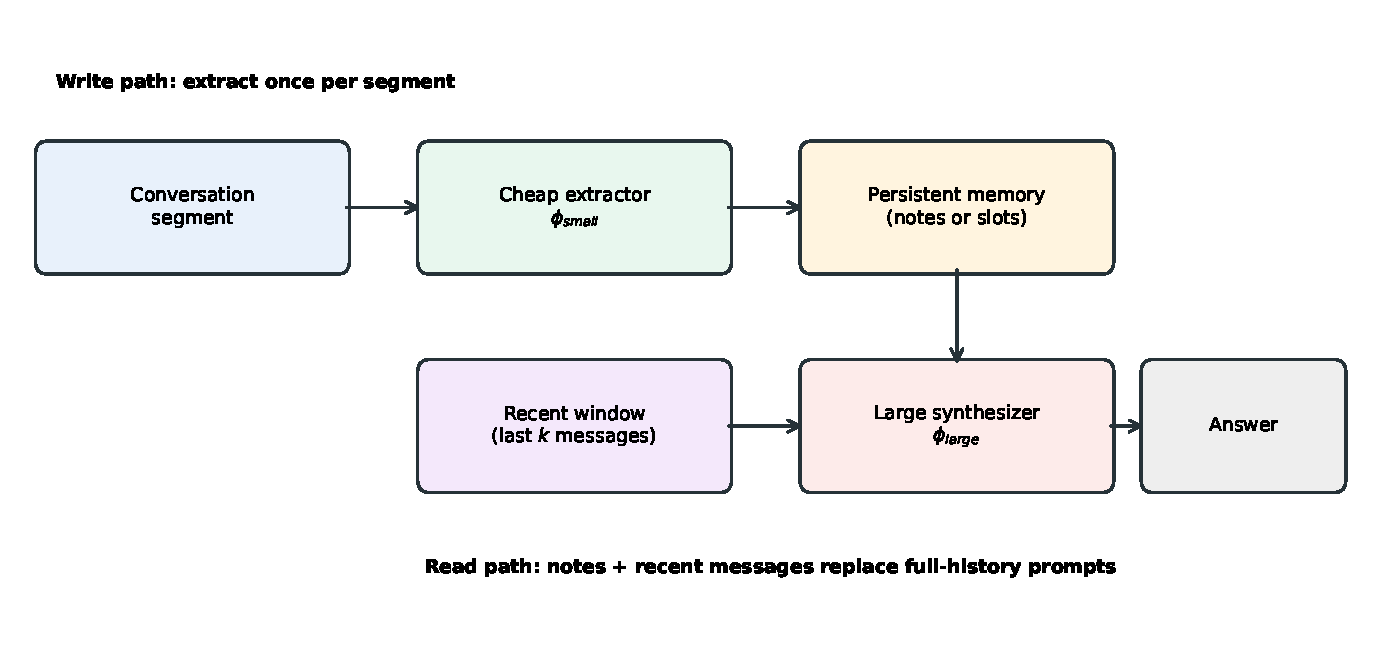
\includegraphics[width=\columnwidth]{architecture_flowchart.pdf}
\caption{Hierarchical memory architecture.}
\label{fig:architecture}
\end{figure}

\begin{algorithm}[h]
\caption{Hierarchical Conversation Management}
\label{alg:hierarchical}
\begin{algorithmic}[1]
\REQUIRE Conversation segment $M = \{m_1, \dots, m_k\}$, Notes file $\mathcal{N}$
\ENSURE Updated notes $\mathcal{N}'$, Response $r$
\STATE $\text{key\_info} \gets \phi_{\text{small}}(M, \text{prompt}_{\text{extract}})$ \COMMENT{Extract salient information}
\STATE $\mathcal{N}' \gets \mathcal{N} \cup \{\text{key\_info}\}$ \COMMENT{Append to persistent notes}
\STATE $\text{context} \gets \text{concat}(\mathcal{N}', M_{\text{recent}})$ \COMMENT{Build compressed context}
\STATE $r \gets \phi_{\text{large}}(\text{context}, \text{prompt}_{\text{synthesis}})$ \COMMENT{Generate response}
\RETURN $\mathcal{N}', r$
\end{algorithmic}
\end{algorithm}

\subsection{Small Model Extraction}

The extraction prompt $\text{prompt}_{\text{extract}}$ instructs $\phi_{\text{small}}$ to identify:

\begin{equation}
\resizebox{\columnwidth}{!}{$\text{key\_info} = \big\{ \text{entities}, \text{decisions}, \text{facts}, \text{goals}, \text{constraints}, \text{preferences}, \text{action\_items} \big\}$}
\end{equation}

Example extraction prompt:
\begin{quote}
From the following conversation, extract: (1) Key entities mentioned (people, organizations, products), (2) Decisions made, (3) Facts established, (4) User goals and preferences, (5) Action items. Format as structured JSON.
\end{quote}

\subsection{Notes File Format}
\label{sec:notes-format}

The persistent notes file employs a structured JSON format:

\begin{equation}
\mathcal{N} = \left\{ n_t = \begin{bmatrix}
\text{timestamp}: t \\
\text{segment\_id}: s_t \\
\text{entities}: E_t \\
\text{decisions}: D_t \\
\text{facts}: F_t \\
\text{goals}: G_t \\
\text{action\_items}: A_t
\end{bmatrix} \right\}_{t=1}^{T}
\end{equation}

Each entry $n_t$ represents extracted information from conversation segment $t$, enabling temporal organization and retrieval.

\subsection{Latest-Value Fact Slots}
\label{sec:slot-format}

The first live evaluation showed that append-only notes can grow too quickly and can preserve obsolete facts. We therefore add a second, deliberately simple representation: latest-value fact slots. Each extracted fact is normalized as

\begin{equation}
f_t = (\text{subject}, \text{predicate}, \text{value}, \text{timestamp}, \text{evidence}).
\end{equation}

The memory table is keyed by $(\text{subject}, \text{predicate})$. When a later segment states a new value for the same key, the system overwrites the old value while keeping a lightweight event log for reproducibility. At read time, the prompt contains only the current slot table plus the recent window. This representation is less general than free-form notes, but it is better matched to fact-tracking conversations with updates such as changed dates, owners, budgets, or priorities. It also provides an explicit mechanism for resolving contradictions by timestamp, a failure mode of append-only notes.

\subsection{Model Selection}

The architecture is model-agnostic, but the empirical results in this paper use a specific Groq-hosted Llama cascade:
\begin{itemize}
    \item \textbf{Small extractor} ($\phi_{\text{small}}$): \texttt{llama-3.1-8b-instant}
    \item \textbf{Large synthesizer} ($\phi_{\text{large}}$): \texttt{llama-3.3-70b-versatile}
\end{itemize}

More generally, the intended configuration is a cheaper extractor paired with a more capable synthesizer, analogous to model-cascade systems such as FrugalGPT \cite{chen2023frugalgpt}. A favorable price ratio is necessary but not sufficient: the notes representation must also retain the facts needed for downstream answering and remain small enough to offset extractor maintenance.

\section{Experimental Design}
\label{sec:experiments}

\subsection{Dataset Generation}

The released generator supports multiple deterministic suites. The full
\texttt{paper} suite contains 20 synthetic conversation test cases:
\begin{itemize}
    \item \textbf{Short}: 14 messages (n = 7)
    \item \textbf{Medium}: 32 messages (n = 7)
    \item \textbf{Long}: 60 messages (n = 6)
\end{itemize}

Topics include product development, research planning, travel booking, technical debugging, and business strategy. Each conversation includes embedded critical information (entities, decisions, facts) for retention evaluation.

For the live Groq results in Section~\ref{sec:results}, we use the smaller
API-cost-controlled \texttt{small} suite. Each seed contains 8 conversations: 3
short (14 messages), 3 medium (30 messages), and 2 long (56 messages). The
append-only notes pilot uses seeds 7 and 8 ($n=16$). The follow-up fact-slot
pilot uses seeds 9 and 10 ($n=16$) and stores raw per-case metrics for paired
analysis.

For deterministic cost-growth analysis, the released generator also includes a stress tier with 120, 240, and 480-message conversations. This tier is used only for local token-accounting simulation unless live API credentials are supplied.

\subsection{Evaluation Metrics}

\begin{table}[h]
\centering
\caption{Evaluation Metrics}
\label{tab:metrics}
\small
\setlength{\tabcolsep}{3pt}
\begin{tabular}{p{0.28\columnwidth}p{0.64\columnwidth}}
\toprule
\textbf{Metric} & \textbf{Definition} \\
\midrule
Token Reduction (real) & $\frac{\text{tokens}_{\text{full}} - \text{tokens}_{\text{method}}}{\text{tokens}_{\text{full}}} \times 100\%$ (provider \texttt{usage}) \\
Token Reduction (cumul.) & Same, via \texttt{tiktoken}/\texttt{cl100k} (growth-curve approximation) \\
Cost (relative) & $\frac{\text{cost}_{\text{synth}} + \text{cost}_{\text{maint}}}{\text{cost}_{\text{full}}} \times 100\%$ \\
Retention Accuracy & $\frac{\text{correct\_answers}}{\text{total\_questions}}$ (containment match) \\
Update Retention & Retention on facts overridden mid-conversation \\
Latency Overhead & $\text{time}_{\text{hierarchical}} - \text{time}_{\text{full}}$ \\
\bottomrule
\end{tabular}
\end{table}

\subsection{Comparison Baselines}
\label{sec:baselines}

We compare against five approaches:
\begin{enumerate}
    \item \textbf{Full Context}: Retain entire conversation history
    \item \textbf{Truncation}: Keep only last $k = 10$ messages
    \item \textbf{LangChain Summarization}: Automatic summarization via same model \cite{acl2024}
    \item \textbf{Append-only Notes}: Hierarchical memory with small model extractor and JSON notes
    \item \textbf{Fact-Slot Memory}: Latest-value slot table extracted by the small model
\end{enumerate}

\section{Results}
\label{sec:results}

We evaluated the system using the Groq inference API with \texttt{llama-3.1-8b-instant} as the extractor ($\phi_{\text{small}}$) and \texttt{llama-3.3-70b-versatile} as the synthesizer ($\phi_{\text{large}}$). This is a pilot-scale evaluation, not a definitive statistical study. Token counts are reported via two methods: per-query ``real'' counts from the provider's \texttt{usage} field (exact, billed), and cumulative counts via \texttt{tiktoken}/\texttt{cl100k} (approximate, for growth-curve shape). Retention is measured by containment-based question answering on planted facts. Cost includes both synthesis tokens and maintenance overhead (extractor calls or summary regeneration).

The initial append-only notes pilot used seeds 7 and 8 ($n=16$) and produced a negative short-horizon result: hierarchical notes retained 69.4\% of planted facts at 102.7\% of full-context cost. Because that representation was not competitive with full context, we added per-case metrics and implemented the fact-slot memory of Section~\ref{sec:slot-format}. Table~\ref{tab:results} reports the follow-up slot-memory pilot on seeds 9 and 10 ($n=16$). Summary intervals in the aggregate artifact are still normal approximations for table readability, while the raw per-case rows are released and used for paired comparisons.

\begin{table}[h]
\centering
\caption{Follow-up Measured Performance with Fact-Slot Memory (n = 16 conversations across two live reruns, $\le$56 messages)}
\label{tab:results}
\scriptsize
\setlength{\tabcolsep}{3pt}
\begin{tabular}{lcccc}
\toprule
\textbf{Method} & \textbf{Token$\downarrow$} & \textbf{Ret.} & \textbf{Upd. Ret.} & \textbf{Cost} \\
\midrule
Full Context & 0.0\% & 95.6\% & 93.8\% & 100.0\% \\
Truncation ($k{=}10$) & 50.8\% & 35.4\% & 37.5\% & 70.2\% \\
Running Summary & 20.1\% & 100.0\% & 100.0\% & 159.8\% \\
Append-only Notes & 19.2\% & 75.7\% & 87.5\% & 103.9\% \\
Fact-Slot Memory & 40.9\% & 85.2\% & 71.9\% & 89.1\% \\
\bottomrule
\end{tabular}
\end{table}

Table~\ref{tab:results} shows that fact-slot memory is a more promising representation than append-only notes, but still not a full-context replacement. Against append-only notes in the same follow-up runs, slots improve real token reduction by 21.8 percentage points, improve retention by 9.5 percentage points, and reduce cost by 14.9 percentage points. Against full context, slots reduce real input tokens by 40.9\% and cost by 10.9 percentage points, but lose 10.4 retention points and 21.9 update-retention points. Against truncation, slots recover 49.8 retention points at 18.9 additional cost points. Against running summary, slots are 70.7 cost points cheaper but 14.8 retention points lower. Figure~\ref{fig:frontier} visualizes this pilot frontier. Mean response overhead for the follow-up run was 0.020 s. Absolute extractor spend over the two slot-memory runs was \$0.00254; summary-maintenance spend was \$0.00714.

\begin{figure}[t]
\centering
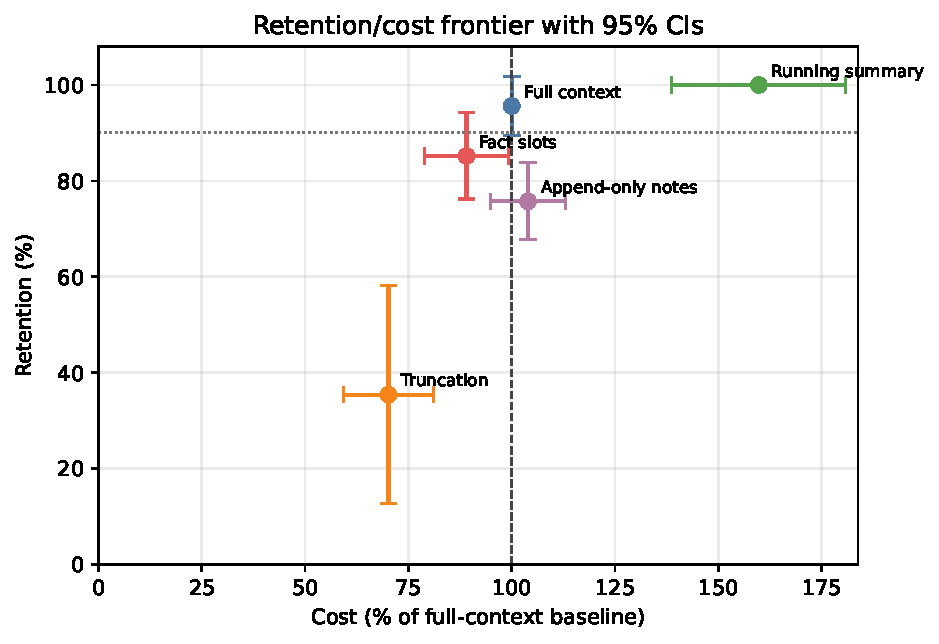
\includegraphics[width=\columnwidth]{retention_cost_frontier.pdf}
\caption{Retention/cost frontier for the follow-up Groq slot-memory runs. Error bars show 95\% intervals from the aggregate summary.}
\label{fig:frontier}
\end{figure}

\subsection{Cascade Ablation: Cheap vs. Expensive Extractor}

To probe the model-cascading hypothesis for append-only notes, we ran an ablation comparing the standard 8B extractor against a 70B extractor (same model as the synthesizer). The ablation held everything else constant: same conversations, same notes schema, same recent window size, same synthesizer. Table~\ref{tab:ablation} reports the result:

\begin{table}[h]
\centering
\caption{Ablation: Extractor Model Size (n = 16)}
\label{tab:ablation}
\small
\setlength{\tabcolsep}{3pt}
\begin{tabular}{p{0.56\columnwidth}c}
\toprule
\textbf{Extractor} & \textbf{Downstream Retention} \\
\midrule
\texttt{llama-3.1-8b-instant} (cheap, 8B) & 69.4\% (CI: [59.6, 79.2]) \\
\texttt{llama-3.3-70b-versatile} (expensive, 70B) & 68.2\% (CI: [59.1, 77.4]) \\
\bottomrule
\end{tabular}
\end{table}

The ablation is statistically inconclusive. The cheap extractor is slightly higher in the pooled point estimate while being far cheaper, but the 1.2 percentage-point gap is small relative to the uncertainty and the intervals almost entirely overlap. We therefore do not claim a quality advantage for the cheap extractor; the result only shows that, in this pilot, the cheap extractor was not obviously worse under this schema and scoring protocol.

\begin{figure}[t]
\centering
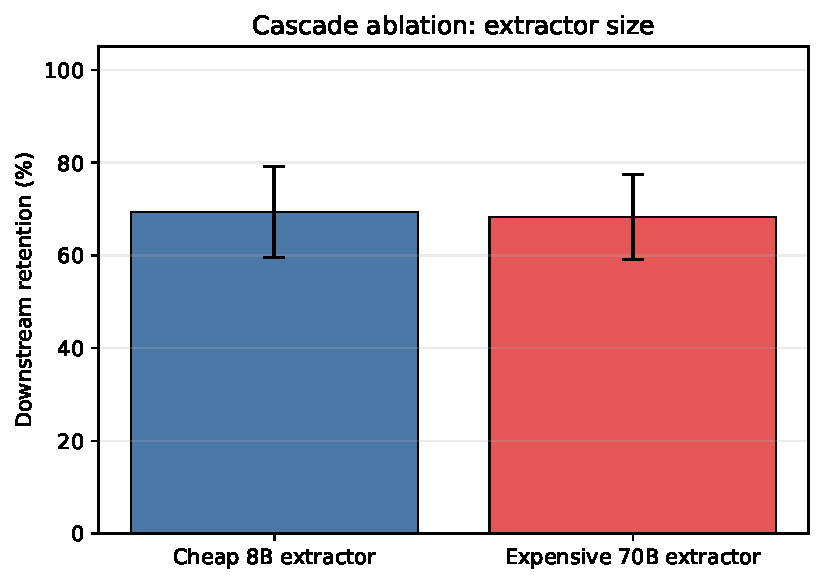
\includegraphics[width=0.92\columnwidth]{cascade_ablation.pdf}
\caption{Extractor-size ablation. The cheap and expensive extractors are statistically indistinguishable in this pilot.}
\label{fig:ablation}
\end{figure}

\subsection{Long-Horizon Token-Growth Simulation}

Because the live run is short, we additionally ran a deterministic token-accounting simulation over 14, 32, 60, 120, 240, and 480-message conversations. This simulation uses the seeded dataset generator, the same context-building code, \texttt{tiktoken}/\texttt{cl100k} local token counts, Groq prices, deterministic offline note extraction, and an optional note-compaction rule that keeps at most 8 notes. It is not a live retention result; it only tests the cost-growth shape. In particular, the 480-message numbers do not show that the system still answers correctly after compaction.

\begin{table}[h]
\centering
\caption{Deterministic Cost vs. Conversation Length (\% of Full Context)}
\label{tab:growth}
\begin{tabular}{rccc}
\toprule
\textbf{Messages} & \textbf{Trunc.} & \textbf{Hier.} & \textbf{Hier. + comp.} \\
\midrule
14 & 96.3\% & 121.7\% & 121.7\% \\
32 & 61.4\% & 91.1\% & 91.1\% \\
60 & 37.7\% & 73.3\% & 71.9\% \\
120 & 20.8\% & 51.9\% & 42.3\% \\
240 & 11.0\% & 42.0\% & 24.0\% \\
480 & 5.7\% & 36.3\% & 13.0\% \\
\bottomrule
\end{tabular}
\end{table}

Figure~\ref{fig:cost-growth} shows the same result as a curve. The simulation suggests that append-only notes are not sufficient for maximum long-horizon efficiency: they beat full context after short warm-up, but bounded notes are far cheaper by 480 messages (13.0\% versus 36.3\% of full-context cost). This is a hypothesis-generating result, not validation. The next necessary experiment is live retention measurement under the same compaction policy.

\begin{figure}[t]
\centering
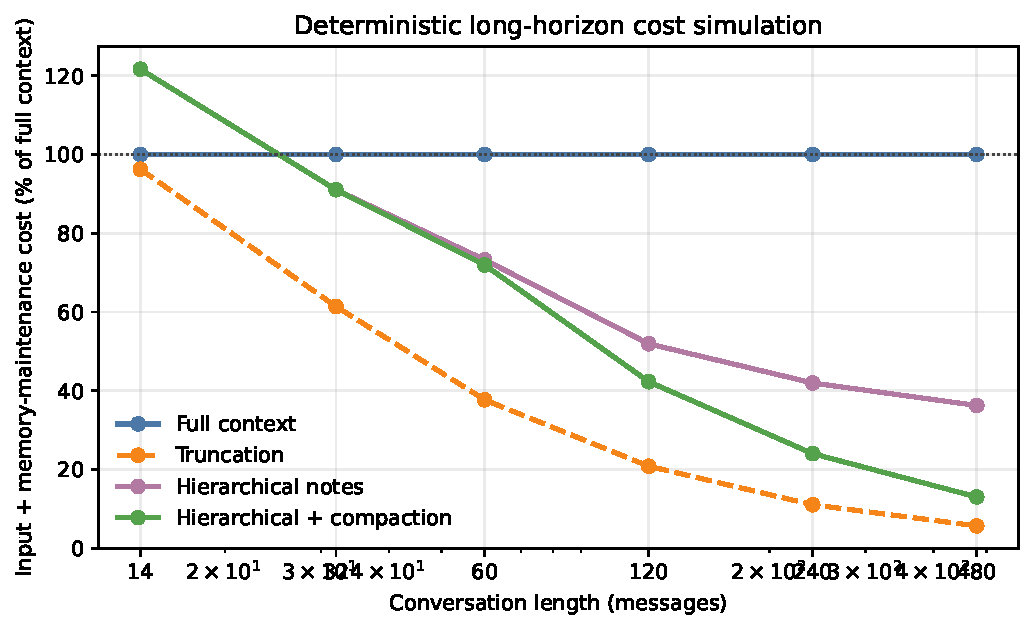
\includegraphics[width=\columnwidth]{cost_vs_length_simulation.pdf}
\caption{Deterministic long-horizon cost simulation. Full context is normalized to 100\% at each length; hierarchical methods include extractor maintenance cost.}
\label{fig:cost-growth}
\end{figure}

Observed properties and open hypotheses:
\begin{itemize}
    \item \textbf{Structured extraction}: The implementation extracts specific categories (entities, decisions, facts), but extraction misses remain a major source of retention loss.
    \item \textbf{Representation choice}: Latest-value fact slots improve the measured frontier over append-only notes, but they are tailored to explicit fact updates and may underrepresent richer narrative context.
    \item \textbf{Model cascading}: Small-model extraction is cheaper \cite{chen2023frugalgpt}, but this pilot does not prove a quality advantage over a large extractor.
    \item \textbf{Persistent memory}: Notes avoid repeated full-summary regeneration, but append-only growth can erase cost gains at short horizons; slot overwrites reduce that growth.
    \item \textbf{Selective context}: Recent messages plus notes can recover more facts than truncation, but did not match full-context retention in the live run.
\end{itemize}

\section{Reference Implementation}
\label{sec:implementation}

To support reproducibility, we release an open-source reference implementation of the architecture described in Algorithm~\ref{alg:hierarchical}. The implementation is a small, dependency-light Python package organized as a research repository, comprising:

\begin{itemize}
    \item \texttt{hierarchical\_memory.py} -- the core memory implementations. It includes append-only structured notes (Section~\ref{sec:notes-format}), latest-value fact slots (Section~\ref{sec:slot-format}), OpenAI-compatible provider clients, robust extraction parsing, and context builders that combine persistent memory with recent messages.
    \item \texttt{token\_utils.py} -- token-counting and reduction utilities built on \texttt{tiktoken}, implementing the Token Reduction and Cost Savings metrics of Table~\ref{tab:metrics}.
    \item \texttt{evaluate.py} -- a harness that runs the baselines of Section~\ref{sec:baselines} over the synthetic conversation suite, supports the long-horizon stress tier, notes compaction, fact-slot memory, and raw per-case metrics, and reports the metrics of Table~\ref{tab:metrics}.
    \item \texttt{make\_figures.py} -- a deterministic artifact generator for the architecture diagram, measured-result plots, and cost-vs-length simulation.
    \item \texttt{scripts/paired\_analysis.py} -- a paired-analysis helper for future evaluator outputs that include raw per-case metrics.
    \item Synthetic conversation generators, a qualitative notes example in \texttt{examples/sample\_notes\_product\_development.json}, pinned dependencies in \texttt{requirements.txt}, a continuous-integration smoke test, and a \texttt{README} documenting setup and usage.
\end{itemize}

The provider interface is abstracted so the small and large models can be backed by any chat-completions-compatible API; the released harness includes both an Anthropic backend and an OpenAI-compatible backend, and the evaluation in Section~\ref{sec:results} was run through the latter against the Groq inference service. Token counts are taken from the provider's own \texttt{usage} accounting rather than estimated with \texttt{tiktoken}, which is an OpenAI tokenizer and mis-counts other model families. The complete source, seeded conversation generator, raw append-only results, raw fact-slot results, paired-analysis outputs, and generated figures are available at \url{https://github.com/sakul7-stack/nodemem}.

\subsection{Research Integrity and Reproducibility}

The evaluation data are generated synthetically by the released code rather than copied from proprietary or copyrighted conversations. The manuscript uses original prose, avoids long quotations, and attributes related methods through the citations in the bibliography. The repository also includes a pre-submission audit script that checks unresolved placeholders, citation coverage, required result artifacts, and accidental API-key leakage. This does not certify acceptance, but it makes the empirical claims and supporting artifacts independently inspectable.

\section{Discussion}

\subsection{Limitations}

\begin{enumerate}
    \item \textbf{Pilot scale and non-dominance}: Each live comparison is only $n=16$ and, at $\le$56 messages, no memory method strictly dominates full context. Append-only notes have similar cost and lower retention; fact-slot memory lowers cost but still loses retention and update accuracy. This is a pilot characterization rather than a proof of token efficiency.

    \item \textbf{Conversation length}: Live retention results are at $\le$56 messages. The deterministic simulation in Table~\ref{tab:growth} supports the expected cost-growth shape, but it does not measure live answer quality. Longer live evaluations ($>$100 messages) are needed to jointly demonstrate cumulative token wins and retention.

    \item \textbf{Extraction errors}: Small model may miss critical information. \textit{Mitigation}: Use high-quality extraction prompts with explicit examples, validate with human review on critical conversations.

    \item \textbf{Information contradiction}: Notes may accumulate conflicting information over time. Fact slots implement timestamp-based overwrite semantics, but their update retention is still weak in the follow-up run (71.9\%). \textit{Mitigation}: add stronger contradiction detection, extractor self-checks, and typed schemas for dates, owners, budgets, and preferences.

    \item \textbf{Tokenizer mismatch}: Cumulative token counts use \texttt{tiktoken} (OpenAI) on Llama outputs and are approximate. Real per-query counts use the provider's own \texttt{usage} and are exact.

    \item \textbf{Statistical power}: The append-only aggregate reconstructs intervals from run-level summaries rather than raw per-case rows, so paired tests cannot be applied retroactively. The fact-slot aggregate stores raw case metrics and supports paired tests, but the current statistics remain underpowered.

    \item \textbf{File growth}: Append-only notes grow indefinitely. \textit{Mitigation}: The reference implementation now includes deterministic notes compaction and fact-slot overwrites, but production systems should use retrieval or learned compaction with explicit conflict handling \cite{karpukhin2020dense}.
\end{enumerate}

\subsection{Future Work}

\begin{itemize}
    \item \textbf{Longer-horizon live evaluation}: Run the new $>$100-message stress tier with live models to measure retention and cost simultaneously. Current live results do not validate a cost-saving claim; the deterministic simulation supports only the cost-growth direction.
    \item \textbf{Retention under compaction}: Measure QA retention with the same bounded-note policy used in the 480-message cost simulation. This is the highest-risk untested component.
    \item \textbf{Slot-memory extraction quality}: Improve the fact-slot extractor with typed schemas, conflict-aware verification, and targeted regeneration for updated facts. Update retention is currently the weakest slot-memory metric.
    \item \textbf{Larger sample and paired tests}: Increase to at least 50--100 conversations per condition, store raw per-case metrics, and report paired method-vs-baseline tests and effect sizes.
    \item \textbf{Vector database integration}: Replace file-based notes with vector store (e.g., ChromaDB, FAISS) for semantic retrieval \cite{karpukhin2020dense}
    \item \textbf{Adaptive extraction}: Dynamically adjust extraction granularity based on conversation complexity using uncertainty estimation
    \item \textbf{Multi-agent coordination}: Share notes across collaborative agents for coordinated task execution \cite{zhou2024agents}
    \item \textbf{Real-world deployment}: Test on production AI agent systems with 1,000 plus conversations to validate enterprise scalability
    \item \textbf{Cross-domain generalization}: Evaluate on diverse domains (healthcare, legal, education) to assess transferability
\end{itemize}

\section{Conclusion}

This paper presents and evaluates a hierarchical memory architecture that applies model cascading to the memory-write step: a cheap extractor maintains persistent structured memory, and an expensive model synthesizes responses from that memory plus a short recent-message window. The initial append-only notes pilot does not establish the architecture as a cost-saving replacement for full context. On synthetic fact-tracking conversations ($\le$56 messages), append-only hierarchical notes retain 69.4\% of facts at 102.7\% of full-context cost. The method is better than truncation on retention but is not competitive with full context in the measured regime. The extractor-size ablation is also inconclusive: cheap and expensive extractors differ by only 1.2 percentage points with overlapping intervals.

A follow-up latest-value fact-slot representation improves the short-horizon frontier: in two additional live seeds ($n=16$), it retains 85.2\% of facts at 89.1\% of full-context cost and reduces real input tokens by 40.9\%. This is a useful pilot signal, especially compared with append-only notes, but it still loses retention relative to full context and remains weak on updated facts. The positive case for persistent memory therefore remains conditional. A deterministic cost simulation shows that bounded notes could reach 13.0\% of full-context cost at 480 messages, but that result is retention-blind and depends on compaction. We release the architecture, seeded generator, raw artifacts, fact-slot variant, and improved evaluator as a transparent pilot study and a starting point for the necessary next experiments: long-horizon live runs, retention under compaction, larger $n$, and paired statistical tests.

\section*{Acknowledgment}

The authors thank Tribhuvan University and the Institute of Engineering for academic support. This research was conducted independently without external funding.

\begin{thebibliography}{99}

\bibitem{packer2023memgpt}
C. Packer, S. Wooders, K. Lin, V. Fang, S. G. Patil, I. Stoica, and J. E. Gonzalez, ``MemGPT: Towards LLMs as operating systems,'' \textit{arXiv preprint arXiv:2310.08560}, 2023.

\bibitem{jiang2023llmlingua}
H. Jiang, Q. Wu, C.-Y. Lin, Y. Yang, and L. Qiu, ``LLMLingua: Compressing prompts for accelerated inference of large language models,'' in \textit{Proc. Conf. Empirical Methods in Natural Language Processing (EMNLP)}, 2023, pp. 13358--13376.

\bibitem{nfliu2023lost}
N. F. Liu, K. Lin, J. Hewitt, A. Paranjape, M. Bevilacqua, F. Petroni, and P. Liang, ``Lost in the middle: How language models use long contexts,'' \textit{Trans. Assoc. Comput. Linguistics (TACL)}, vol. 12, pp. 157--173, 2024.

\bibitem{zhang2024memorysurvey}
Z. Zhang, X. Bo, C. Ma, R. Li, X. Chen, Q. Dai, J. Zhu, Z. Dong, and J.-R. Wen, ``A survey on the memory mechanism of large language model based agents,'' \textit{ACM Trans. Inf. Syst.}, 2024. (Also \textit{arXiv preprint arXiv:2404.13501}.)

\bibitem{acl2024}
M. Sung, S. Lee, J. Kim, and S. Kim, ``Context-aware LLM translation system using conversation summarization and dialogue history,'' in \textit{Proc. 9th Conf. Machine Translation (WMT)}, 2024, pp. 1011--1015.

\bibitem{park2023generative}
J. S. Park et al., ``Generative agents: Interactive simulacra of human behavior,'' in \textit{Proc. 36th Annual ACM Symposium on User Interface Software and Technology (UIST)}, 2023, pp. 1--22.

\bibitem{shinn2023reflexion}
N. Shinn et al., ``Reflexion: Language agents with verbal reinforcement learning,'' in \textit{Advances in Neural Information Processing Systems (NeurIPS)}, vol. 36, 2023.

\bibitem{zhou2024agents}
S. Zhou et al., ``WebArena: A realistic web environment for building autonomous agents,'' in \textit{Proc. International Conference on Learning Representations (ICLR)}, 2024.

\bibitem{chen2023frugalgpt}
L. Chen et al., ``FrugalGPT: How to use large language models while reducing cost and improving performance,'' \textit{arXiv preprint arXiv:2305.05176}, 2023.

\bibitem{zhong2024memorybank}
W. Zhong et al., ``MemoryBank: Enhancing large language models with long-term memory,'' in \textit{Proc. AAAI Conference on Artificial Intelligence}, 2024.

\bibitem{bang2023gptcache}
F. Bang, ``GPTCache: An open-source semantic cache for LLM applications enabling faster answers and cost savings,'' in \textit{Proc. 3rd Workshop for Natural Language Processing Open Source Software (NLP-OSS)}, 2023, pp. 212--218.

\bibitem{karpukhin2020dense}
V. Karpukhin et al., ``Dense passage retrieval for open-domain question answering,'' in \textit{Proc. Conference on Empirical Methods in Natural Language Processing (EMNLP)}, 2020, pp. 6769--6781.

\end{thebibliography}

\end{document}